\section{Discussion and conclusions}
\label{sec:discussion}
We have four topics to discuss here:
\begin{itemize}
\item \textbf{Velocity map binning methods:} a technical discussion on the comparative merits of alternative MaNGA velocity map binning methods and IFU sizes to obtain best resolution Radon profile traces.
\item \textbf{Correlation between Radon profiles classes and morphology:} we discuss a possible relationship between Radon transform trace profile Types and galaxy morphology.
\item \textbf{Findings and conclusions:} a review of the significant findings of the project and presentation of our conclusions.
\item \textbf{Future work:} some topics for future work noted during the course of the project. 
\end{itemize}

\subsection{Velocity map binning methods}
\label{sec:binning-methods}
The MaNGA DAP utilises various spaxel binning models to process the IFU fibre bundle data into the output maps. The available binning schemes used to produce gas and stellar velocity maps, together with a brief description of each are listed below.

\begin{itemize}
    \item SPX - single spaxel measurements i.e. no binning.
    \item VOR10 - Voronoi binning, an adaptive spatial binning method where low signal-to-noise (S/N) ratio spaxels are grouped to achieve an overall S/N of 10  \citep{2003MNRAS.342..345C, 2019arXiv190100856W}.
    \item HYB10 - Hybrid binning: Voronoi S/N 10 binning for stellar velocity maps, but unbinned for emission line properties which are used to generate gas velocity maps.
\end{itemize}  

In this study we have utilised MaNGA datacubes released in DR15 MPL-7 which have been processed in the DAP using the hybrid HYB10 binning model, i.e. using VOR10 binning for the stellar velocity maps. However, the MaNGA project team currently have an internal dataset available, MPL-8. Datacubes in MPL-8 include VOR10 and SPX binning schema. We were interested to make a comparison of the Radon trace profiles generated from the datacubes using the Voronoi and SPX binning schemas. A limited sample of MPL-8 cubes were made available for this comparison exercise. We selected 2 galaxies from our samples with stellar velocity maps having poor spatial definition, and another 2 with good resolution in order to compare the Radon transform profiles using the Voronoi binning and SPX (unbinned) methods. The selected datacubes were firstly, examples of good resolution/definition in stellar velocity maps:

\begin{itemize}
    \item 7977-12704
    \item 8322-1901
\end{itemize}

and secondly, examples of poor resolution/definition in stellar velocity maps, i.e. having a blotchy appearance, due to spatial binning of low S/N spaxels, or with masked spaxels:

\begin{itemize}
    \item 9088-12703
    \item 8993-6104
\end{itemize}

The stellar velocity maps together with their Radon transform and trace profiles for these well defined example 7977-12704 are shown in Figure \ref{fig:binning-comparison}. The differences being the binning models of the input stellar velocity maps: Voronoi binning in the left-hand panel and SPX binning on the right. A comparison shows that there is little difference in the Radon transform and Radon profile plots. It is also apparent that the Radon transform algorithm for the SPX velocity maps yields a greater number of valid data points in the trace plot. We conclude that both VOR10 and SPX binned maps would lead to the same Type classification in these cases. This conclusion was also obtained for other galaxy showing good resolution in the stellar velocity map,  8322-1901 (figure not included). 

However, the same conclusion does not apply for the low resolution stellar velocity map examples, 8993-6104 shown in Figure \ref{fig:binning-comparison2} and 9088-12703 (figure not included). In these cases, at first sight, there are marked differences in the extent of spatial coverage and shapes of the velocity field PA, the Radon transform minimum and the Radon profile. In particular the control galaxy 8993-6104 displays a clearly asymmetric Radon profile with VOR10 binning, but could possibly be interpreted as an outer bend in the Radon profile trace of the SPX map. However, on closer inspection, looking at the  range the trace plots, the same bend feature at Radon transform coordinates [$\rho$, $\theta$]=[-6,+2],[20, 50] is apparent in both binning model plots. The asymmetric feature at $\rho$ \textgreater\ +2 apparent in the left Voronoi binned trace is not evident in the SPX output shown in the right-hand panel. Although these differences can be expected due to the exclusion of low S/N low spaxels in the SPX maps, crucially this can easily lead to a different visual classification result between the transforms of Voronoi binned and SPX velocity field maps. 
\begin{figure*}
    \centering
    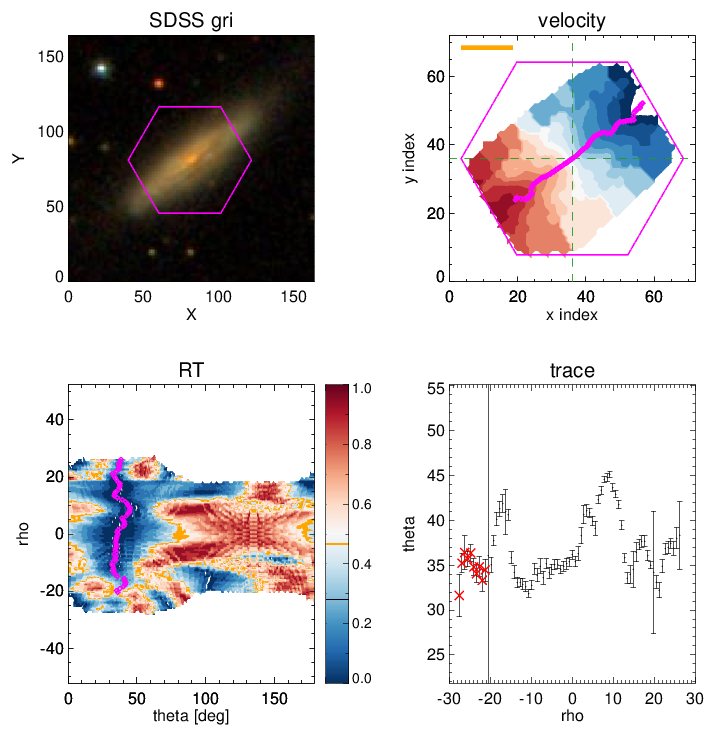
\includegraphics[width=\columnwidth]{images/RadonPlots/RT-SNIPS-NEW/7977-12704-VOR10-MILESHC-MILESHC-1-SNIP.png}
    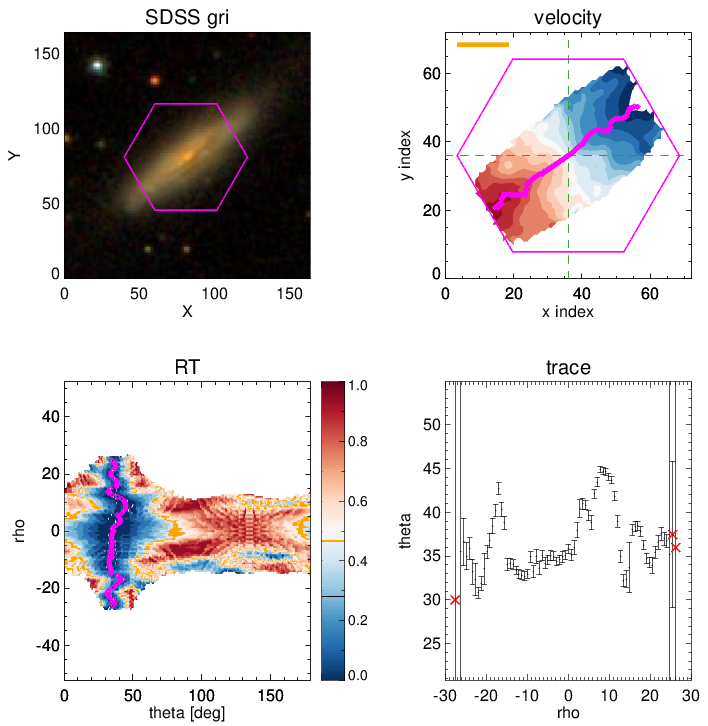
\includegraphics[width=\columnwidth]{images/RadonPlots/RT-SNIPS-NEW/7977-12704-SPX-MILESHC-MILESHC-1-SNIP.png}
    \caption[Comparison of velocity map binning schemes for a high resolution map]{Comparison of stellar velocity map binning methods using the Radon transform output graphic for the galaxy 7977-12704. The velocity map has good resolution using both schemes. In the left panel the transform RT and profile trace plots are generated from the stellar velocity map with Voronoi binning. The plots in the right panel were produced from the stellar velocity map using single spaxel SPX resolution. The layout of the 4 subplots in each panel is as described in Figure \ref{fig:8442-3704-complete}.}
    \label{fig:binning-comparison}
\end{figure*}

\begin{figure*}
    \centering
    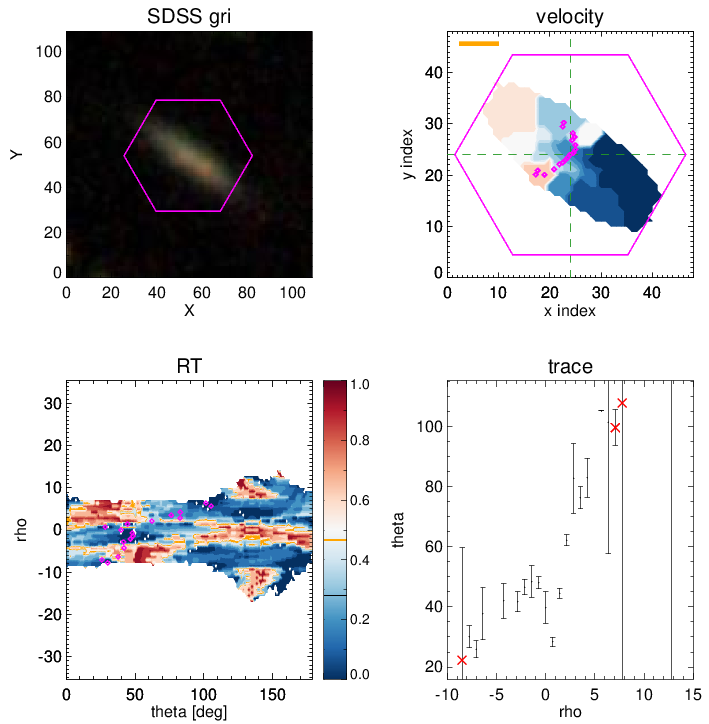
\includegraphics[width=\columnwidth]{images/RadonPlots/RT-SNIPS-NEW/8993-6104-VOR10-MILESHC-MILESHC-1-SNIP.png}
    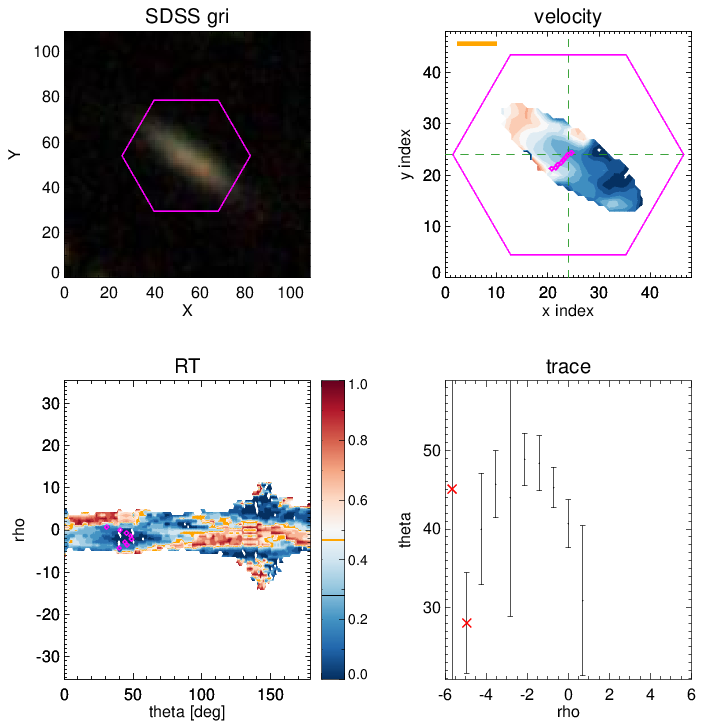
\includegraphics[width=\columnwidth]{images/RadonPlots/RT-SNIPS-NEW/8993-6104-SPX-MILESHC-MILESHC-1-SNIP.png}
    \caption[Comparison of velocity map binning schemes for a low resolution map]{Comparison of velocity map binning schemes for a low resolution map. Radon transform output graphic for the galaxy 8993-6104 with a low resolution stellar velocity map. In the left panel the transform RT and profile trace plots are generated from the stellar velocity map with Voronoi binning. The plots in the right panel were produced from the stellar velocity map using single spaxel SPX binning. The layout of the 4 subplots in each panel is as described in Figure \ref{fig:8442-3704-complete}.}
    \label{fig:binning-comparison2}
\end{figure*}




\subsection[Correlation between Radon profiles and morphology]{Correlation between Radon profile types and morphological features}
\label{sec:correlations}
\cite{2018MNRAS.480.2217S} made considerable efforts to explore  possible correlations between the observed frequencies of the 5 Radon profile types (Type-C, Type-A, Type-IB, Type-OB and Type-OB+IB) and underlying morphological features obtained from the Galaxy Zoo morphology classification project. They found some evidence of associations between Radon profile trace type and morphological features, as discussed in detail in their paper, Section 5. These correlations are subjective, however, and certainly not exclusive of other possible interpretations of Radon type to morphology relationships. We stress that Care must be taken to follow their arguments closely. In our opinion, the most assertive of those relationships can be broadly summarised as follows:
\begin{itemize}
\item Type-C: Constant profile - apparent in unbarred galaxies.
\item Type-A: Asymmetric profile - often associated with tidal interactions.
\item Type-IB: Inner bends - prevalent in strongly barred galaxies.
\item Type-OB: Outer bends - often associated with kinematic warps.
\end{itemize}

Following the above interpretation there are two relevant points to to the discussion. Firstly that Radon profile Type-OB outer bend features have an association with kinematic warps. In this way Type-OB profiles could represent the signatures of past mergers in disc galaxies. Secondly, if Radon Type-A asymmetric profiles are associated with tidal interactions and tidal tails, then Type-A profiles may represent the signatures of gas-poor, dry mergers in early-type galaxies, see e.g.  \cite{2005AJ....130.2647V}. 

%%%% ====================================

%%% Stopping here for the night ...

%%% =====================================

As reported in our results Section \ref{sec:comparison-of-results} we found that 5 out of 14 PSBs with large $\Delta$PA$_{k}$ offsets were assigned Radon profile trace classification of Type-OB. We emphasise that this result was determined by Classifier A, and there was little consensus with the classifications of either Classifier B, or in the limited number of automatic classifications that were available for our galaxies. Setting this point aside for now, some correlation may exist between Radon outer bend profiles, large $\Delta$PA$_{k}$ and past major mergers. Again we stress that much further work is required to provide consistent interpretations of Radon profile trace types before we can make this conclusion.

\subsection{Findings and conclusions}
\label{findings}

In our analysis of kinematic position angle offsets we have shown that CPSBs possess a wide range of $\Delta$PA$_{k}$ above 30\textdegree\ with many greater than 90\textdegree. RPSBs have a smaller range in $\Delta$PA$_{k}$, with only a few over 90\textdegree. The majority of control galaxies have small kinematic position angle differences, clustered at less than 25\textdegree. Significant misalignment in the gas and stellar velocity fields of CPSBs, and to a lesser extent in RPSBs, reveal kinematic disturbances indicative of past major mergers.
We noted that the distribution in $\Delta$PA$_{k}$ is markedly different when comparing CPSBs with the CPSB control set, and this trait is present, but to a lesser degree in the comparison of the RPSB $\Delta$PA$_{k}$ with their controls. The distribution in  kinematic position angle offsets is similar for both control sets. These observations are strongly supported by the results of K-S analysis in Section \ref{sec:K-S-test} where we found the difference in $\Delta$PA$_{k}$ of both PSB groups, as compared to their control groups, to be statistically significant. In summary, the most significant finding arising from the kinematic position analysis study is that there is a combination of mutually supportive evidence of past disruption derived from the properties of PSBs, and we can concluded that mergers play a role in galaxy evolution. This evidence was identified in three topics: the $\Delta$PA$_{k}$ distributions in the CPSB, RPSB and their control sets; the supporting K-S statistical analysis performed on these $\Delta$PA$_{k}$ distributions; and the differences in distributions of S\'ersic index. Taken together these indicators point towards an evolutionary sequence from normal, non-PSB (control) galaxies, to the lower S\'ersic index disc-like RPSBs, and on to the redder spheroidal CPSBs with higher S\'ersic indices. We see PSBs as the indicators of morphological transition from late-type disc galaxies to red spheroids depicting an evolutionary pathway from the blue cloud, through the green valley, towards the red sequence.

Before we present the main results of the Radon transform method, we summarise the technical discussion comparing the relative merits of MaNGA map binning schema and IFU size. We compared the Radon profile trace results obtained from stellar velocity maps employing Voronoi VOR10 binning versus the single spaxel SPX unbinned schema. We obtained cleaner trace profiles (i.e. easier to classify) with a greater number of valid data points and tighter error bars from high S/N maps based on single spaxel SPX binning. For future studies, given a large enough sample of PSBs, we should avoid Voronoi binned maps where possible and use SPX maps taking a cut of S/N greater than 3 or more in single spaxels.

A substantial effort was put into the visual classification of  Radon transform profile trace plots of the stellar velocity maps to determine their trace feature Types.  It was noted that visual classification was difficult. Our classifiers agreed on this point. In addition, our classifiers arrived at disparate, sometimes opposing interpretations of profile type class for most galaxies, even though the same written classification procedure was followed. We now recognise the difficulties in relating the trace plots to the 'standard' examples. With only two participating classifiers we conclude that there must be significant classification error present in our results, recalling that the Galaxy Zoo project engaged $\sim10^5$ classifiers to minimise classification error.

We compared the results of the kinematic PA analysis with those the Radon transform analysis technique. As mentioned in Section \ref{sec:motivation} the Radon transform method should provide distinct advantages over the kinematic $\Delta$PA$_{k}$ method. Radon transforms provide a detailed trace of position angle across the velocity field enabling local regions of radial variation to be identified. Kinematic PAs require both stellar and gas velocity fields to be mapped but post-starburst galaxies may possess little gas. The Radon transform can identify local regions of disturbance, as evidence of merger activity, using the stellar velocity field alone.

Earlier in this discussion (Section \ref{sec:correlations}) we put forward the notion that Radon profile Type-OB features may be consistent with kinematic warps in stellar discs, while Type-A profiles suggest the presence of tidal tails from interacting or merged early-type field galaxies. In both cases merged systems of sufficient age, 1 to 2 Gyr, will reveal the characteristics of post-starburst galaxies. We suggested that Radon trace profiles displaying outer bends, Type-OB or Type-OB+IB (indicating warped stellar discs) could be considered prospective candidates of past major mergers in disc-dominated systems, while Type-A profiles (consistent with tidal interactions) may correlate with ongoing or past mergers in elliptical systems. From Table \ref{tab:Radon-VC-results} we saw that Classifier A identified 10 of of 27 CPSBs (37\%), and 10 out of 36 RPSBs (28\%) as having Type-OB or Type-OB+IB Radon profile signatures. Type-A features were evident in  15\% of CPSBs and 19\% of RPSBs. If this classification is reliable, and the correlation between type and morphology is valid (there are considerable uncertainties in both these areas), then we could conclude that there is some evidence of past mergers in post-starburst galaxies. This tentative conclusion needs to be supported by further research into the areas of uncertainty: Radon profile classification and the correlation relationship between Radon type and morphology.

% \subsection{Summary}
% \label{summary}
In previous studies major mergers have been detected using imaging techniques. In this project we have attempted to identify past major mergers in PSB galaxies, firstly by investigating the distributions of differences in stellar and gas velocity field kinematic position angles, and secondly by using the Radon transform method to reveal radial variation in kinematic position angles. 
We obtained a positive result from the $\Delta$PA$_{k}$ analysis revealing that PSBs lie on a evolutionary track between the blue cloud and the red sequence. The Radon transform method, however, did not provide conclusive results. We attribute this to the difficulty in classifying kinematic features from the trace plots. More work is required to provide consistent classification of kinematic features apparent in the Radon profile trace plots. 

It was noted that \cite{2019DDA....5020304N} have recently announced work which promises to increase the accuracy of merger detection using a method that integrates imaging and kinematic analysis techniques. This extended method will combine SDSS imaging (providing morphological observations) with MaNGA  kinematic maps, towards enhanced identification of merger and post-merger signatures. When available, this technique should be applied to our PSB and control samples to provide additional evidence of past mergers in post-starburst galaxies.
